\documentclass{article}
\usepackage[utf8]{inputenc}

\title{Project Proposal: Optical Character Recognition on WHO datasets}
\author{Hanna Rakhsha \and Ram Moore \and Samantha Aziz}
\date{October 1, 2019}

\usepackage{graphicx}
\usepackage{subcaption}
\usepackage{natbib}
\usepackage[section]{placeins}
\graphicspath{ {./images/} }

\begin{document}

\maketitle

\section{Problem Description}
We have been provided with a 140,000 page data set of document scans from a WHO (World Health Organization) database.
Much of the text has been read using OCR software, but due to a combination of poor quality scans and possible unusual typewriter fonts, the OCR software is unusable and the text, unsearchable.
We hope to provide a search-able OCR reading of the documents with the minimum functionality of identifying country names from within the documents.

\section{Introduction}
In the past 20 years products like Adobe Acrobat and Google Drive have made major advancements in optical character recognition.
Most OCRs come out at around 98 to 99 percent accuracy on a full page of translation. \citep{Council}
This incredible feat still manages to come with a few problems.
One of the problems with OCR software is that over a large set of documents the missed characters start to add up.
Moreover, documents that are worse quality or have hard-to-read fonts risk almost a 30 percent difference in accuracy. \citep{Holley}

The data set we are hoping to use is given to us by Dr. Louie Valencia, a Texas State University history professor.
His hope is to further research in the AIDS/HIV epidemic around Europe through the 80s and 90s.
This set contains 1,376 documents, with around 100 pages per document, putting the total data set at around 137,600 pages.
The content of this material range from AIDS research funding requests to reports of tests and research already being done.

Dr. Valencia has requested better OCR software so that he can easily search the documents.
Since he will be focusing his research on the countries that performed the most research, his first step will be using the documents received from the WHO to find which countries had the most correspondence regarding HIV/AIDS.
This is why the minimum functionality of our program will be to pull country names from the data set.
%Do we have access to his current OCR software? Do we know what it is/what algorithm it uses?
%That'd be a question for Ram or i guess email Louie? i have no idea on it
%
%I think we believe that the OCR run on the documents was the OCR that was built into the scanner but I'm not sure, we could ask him about it. -Ram
The problems he has come across with OCR software now are as follows:
\begin{enumerate}
  \item Documents with low quality scans don't get recognized.
  \item Specific typewriter fonts and text sizes/spacing group words together incorrectly and are generally inaccurate.
  \item Hand written notes or pages get missed all together.
\end{enumerate}

We will investigate the weaknesses in Dr. Valencia's current OCR software, develop possible solutions, and implement a comparable machine learning algorithm.
We also plan to compare his current OCR software and our own, to gauge the efficacy of our approach.

The ultimate goal and focus of our project is to identify the source of these shortcomings, and increase the accuracy for worse quality documents and hard-to-read fonts in large data sets.

\section{Preliminary Plan}
%To do: Mention milestones/deliverables
This investigation will occur in three stages.
\begin{enumerate}
  \item Preliminary analysis -- We will first evaluate the shortcomings of Dr. Valencia's current OCR software.
  Correctly identifying the weaknesses in his current implementation is an imperative piece of our investigation, as it will guide the development of our own OCR project.
  \item Algorithm development, training, and testing -- Develop a classification algorithm that will pre-process scanned documents and extract key features of each character detected.
  The algorithm will then analyze these features to classify each character.
  To achieve a high character recognition rate, this algorithm will require a fair amount of fine-tuning, especially because we are attempting to perform OCR on a noisy, unfiltered data set.
 %We can compare our algorithm against Louie's OR an OCR that exists somewhere else, but I'd like to include some performance metric--it will make our algorithm look good :^)
 %This sounds like a great idea! -H
  \item Comparison -- Using our own OCR algorithm, we will perform optical character recognition on a subset of the existing data set.
  We will compare our results to those of another commercially available OCR software that on the same subset.
  We anticipate that, for this particular data set, our OCR software will perform better than Dr. Valencia's current program and perform reasonably well when compared to the commercially available OCR software.
\end{enumerate}

\section{Challenges}
Below are examples of the problems listed in the introduction.
  %Differentiating between random marks on the page (top line: applicable) and accent marks (bottom line: numero)
\begin{figure}[!ht]
  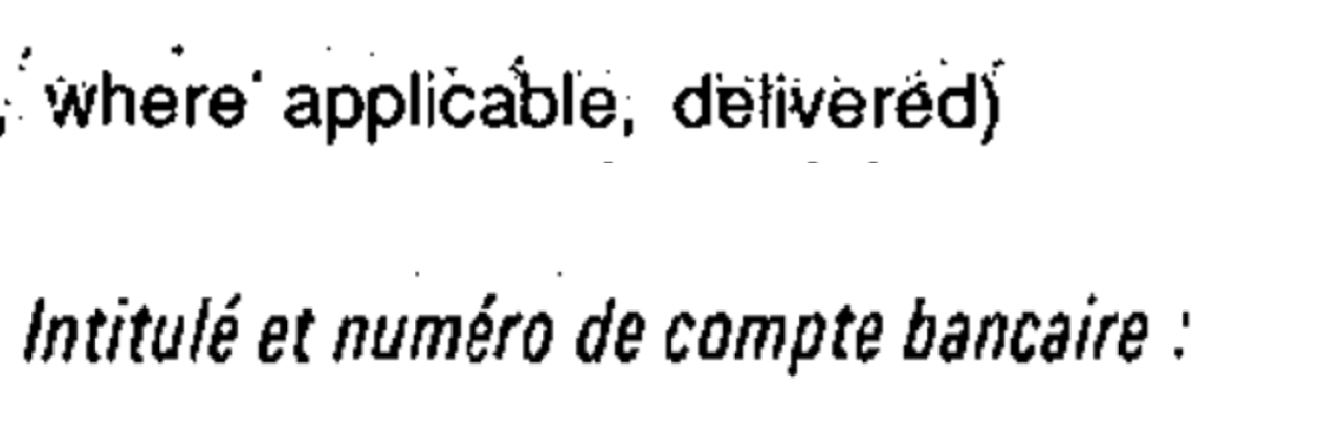
\includegraphics[width=75mm, scale=0.5]{AccentMark_Dirt.png}
  \caption{Example of random marks verses accent marked words.}
  \label{fig:boat1}
\end{figure}

\begin{figure}[!ht]
  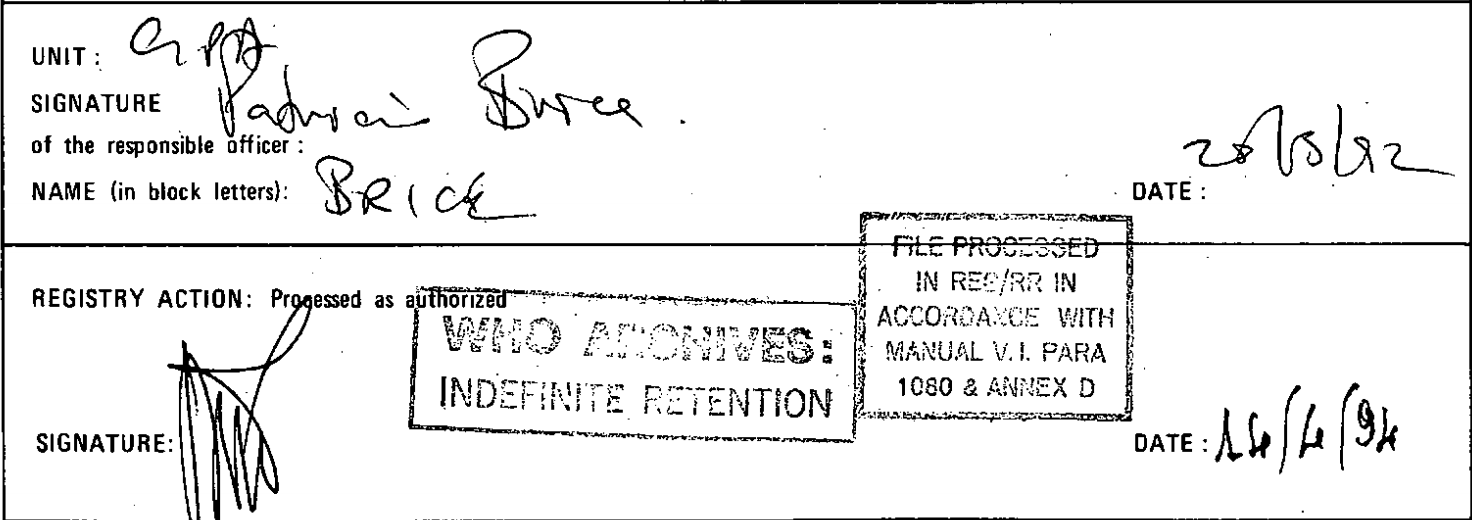
\includegraphics[width=100mm, scale=0.5]{Signature.png}
  \caption{Example of hand writing.}
  \label{fig:boat2}
\end{figure}

\begin{figure}[!ht]
  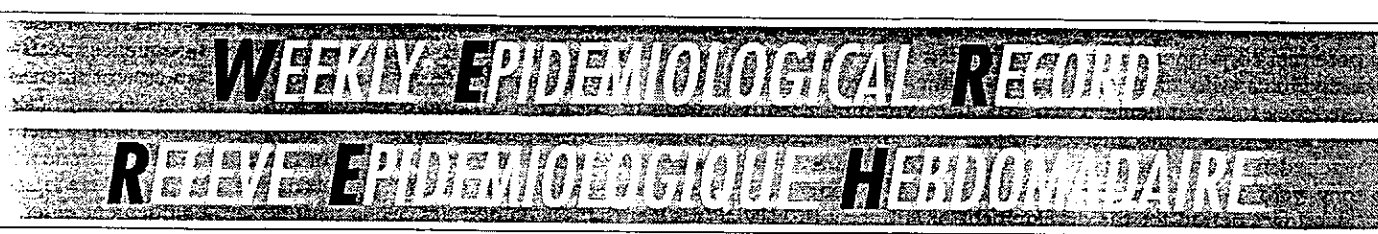
\includegraphics[width=100mm, scale=0.5]{PoorQuality.png}
  \caption{Example of poor quality document.}
  \label{fig:boat3}
\end{figure}

\bibliographystyle{plain}
\bibliography{references}
\end{document}
